% code to pdf: ctrl + alt + j
\chapter{System Model}
\label{chap:model}
% system flow diagram
% satellite orbit pattern
\section{System Overview}

This chapter introduces the LEO satellite communication system, as illustrated in Figure~\ref{fig_system}. We consider one of the satellites in the LEO satellite communication system. It consists of $M$ beams, represented by $\mathcal{M} = \{m\ |\ m = 1, 2, \ldots, M\}$. In the coerage area of the satellite, it contains $K$ cells, indexed by $\mathcal{K} = \{k\ |\ k = 1, 2, \ldots, K\}$. To achieve optimal coverage and minimize overlap, all ground cells are arranged in a regular hexagonal grid, ensuring uniform cell size. There are $U$ user equipments (UEs) in the coverage area, indexed by $\mathcal{U} = \{u\ |\ u = 1, 2, \ldots, U\}$. 

\begin{figure}[h!]
    \centering
    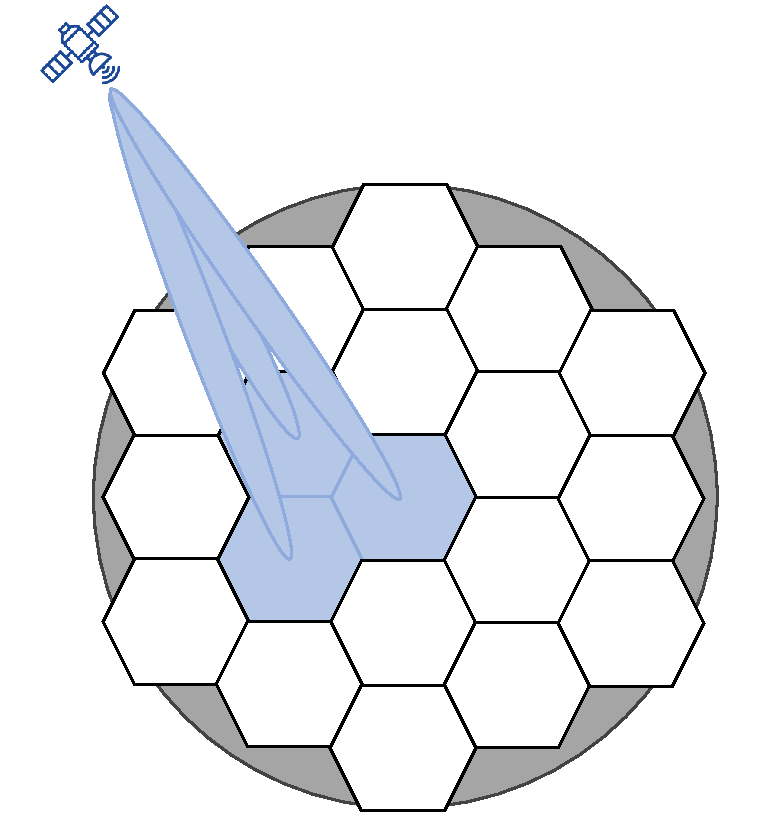
\includegraphics[width=0.8\textwidth]{figure/system overview2.pdf}
    \caption{Illustration of satellite beams and cells.}
    \label{fig_system}
\end{figure}
% TODO: time slot definition
We define a short time $T^{slot}$ as the time duration of a time slot, and $T^{total}$ as the total time that the satellite serves the area. Thus, there are $T^{total} / T^{slot}$ time slots in total service time, denoted as $\mathcal{T} = \{t\ |\ t = 1, 2, \ldots, T^{total} / T^{slot}\}$. 

In this thesis, we adopt the quasi-earth-fixed scheme. Unlike the earth-moving cell scheme—where the coverage areas of satellite beams move as the LEO satellites orbit—this approach directs satellite beams so that each beam consistently covers the same geographical cell for a given period. Thus, the coverage area of each satellite beam remains fixed relative to the ground during that interval. Throughout, we assume each satellite beam is oriented toward the center of its designated cell.

The locations of UEs wishing to access the network are assigned randomly within their corresponding cells, and the population of each cell are generated according to area population density statistics.

\section{Channel Model}

\subsection{Free Space Path Loss}
In the LEO satellite system, the free space path loss from the satellite to cell $k$ is expressed as follows~\cite{Satellite-Multi-Beam}:
\begin{equation}
    L_{k} = \left(\frac{\lambda}{4\pi d_{k}}\right)^2
\end{equation}
where $\lambda$ is the wavelength, and $d_{k}$ is the distance between the satellite and the center of the $k$-th cell.

\subsection{Shadowed-Rician Fading Channel}
The shadowed-Rician fading model is suitable for satellite communication systems because it accurately reflects the physical propagation environment, capturing both the presence of a strong line-of-sight (LoS) signal and the effects of shadowing from obstacles~\cite{channel-model}. Let $h_{k}$ denote the channel gain between the satellite and the $k$-th cell. The cumulative distribution function (CDF) of the channel gain is:
\begin{equation}
    F_{h_{k}}(x) = K \sum_{n=0}^{\infty} \frac{(m)_n \, \delta^n \, (2b)^{1+n}}{(n!)^2} \, \zeta\left(1+n, \frac{x}{2b}\right)
\end{equation}
where $K = \left(\frac{2bm}{2bm+\Omega}\right)^m/2b$, $\delta = \Omega/(2bm+\Omega)/2b$, $\Omega$ is the average power of the LoS component, $2b$ is the average power of the multipath component except the LoS component, and $m$ is the Nakagami parameter.  $\Gamma(\cdot)$ is the Gamma function, and the Pochhammer symbol is defined as $(x)_n=\Gamma(x+n)/\Gamma(x)$. The lower incomplete Gamma function is defined as $\zeta(a, x) = \int_0^x t^{a-1} \exp(-t)dt$.

\subsection{Antenna Radiation Pattern}
We introduce the antenna radiation pattern in~\cite{Energy-Efficient}:
\begin{equation}
    G(\phi_{m,u}) = G_{max} \left[ \frac{J_1\left(\mu(\phi_{m,u})\right)}{2\mu(\phi_{m,u})}
    + 36 \frac{J_3\left(\mu(\phi_{m,u})\right)}{\mu(\phi_{m,u})^3} \right]^2
\end{equation}
where $\phi_{m,u}$ is the boresight angle between the user position and the beam center with respect to the satellite, $G_{max}$ is the maximum antenna gain, $\mu(\phi)$ is defined as $2.07123 \cdot \sin(\phi)/\sin(\phi_{3dB})$, $\phi_{3dB}$ is the 3 dB half-power beamwidth angle of the antenna, and $J_1(\cdot)$, $J_3(\cdot)$ are the Bessel functions of the first kind of orders 1 and 3, respectively.

\subsection{UE Received Power}
In this thesis, the transmitted power of each beam is fixed during one epoch. The transmitted power to the $k$-th cell at the $\mathcal{S}_i$-th epoch is denoted as $P_{k}[\mathcal{S}_i]$. In the $\mathcal{S}_i$-th epoch, the received power of the $u$-th user in the $k$-th cell at the $t$-th time slot $\hat{P}_{k,u}[t]$ can be calculated as follows:
\begin{equation}
    \hat{P}_{k,u}[t] = P_{k}[\mathcal{S}_i] \cdot L_{k} \cdot h_{k} \cdot G(\phi_{k,u}) \label{eq:T-R}
\end{equation}

% We define Signal-to-Noise Ratio (SNR) of the $u$-th UE as follows:
% \begin{equation}
%     SNR_u = \frac{\hat{P}_{m,u}}{N}
% \end{equation}
% where $N$ is the power of the white gaussian noise, which is a random variable with mean $0$ and variance $\sigma$.
\section{Joint Power-Periodicity Optimization on SSB}
In this section, we will discuss how the satellite beam transmitted power and the SSB periodicity affect UE cell search delay and formulate an optimization problem. 
During the total service time, it is essential to adjust the satellite beam transmitted power and the SSB periodicity because the system environment changes in real-time. The most significant change is the elevation angle of the satellite. It affects not only the transmission distance, but also the channel fading effect. However, if we adjust the power and periodicity too frequently, the computation complexity rises and the signaling overhead increases. Thus, we adjust the satellite beam transmitted power and the SSB periodicity in a certain number of time slots, defined as an epoch. We define one epoch equals to $N$ time slots, so there are $T^{total} / T^{slot} / N$ epochs in total. The set of all epochs within the service duration is represented as $\mathcal{\widetilde{S}} = \{\mathcal{S}_i\ |\ i = 0, 1, 2, \ldots, (T^{total} / T^{slot} / N - 1)\}$, where each epoch $S_i$ encompasses the time slots from $iN$ to $(i + 1)N - 1$. By adjusting system parameters only at epoch boundaries, this approach balances real-time responsiveness against the complexity and signaling overhead associated with too frequent updates, ensuring system stability and efficient resource allocation throughout the mission duration.

\subsection{Synchronization Signal Block Periodicity}

During the total service time, the satellite transmits SSBs to the serving cells at specific time intervals, depending on the SSB periodicity configured for each cell. With longer SSB periodicity, the satellite beam has more time slots to serve other cells, and can allocate more power to each SSB signal. Thus, we adjust the SSB periodicity every epoch. During each epoch, the SSB periodicity of each cell is fixed. We then define the SSB periodicity of the cell $k$ at the $\mathcal{S}_i$-th epoch as the number of slots between two consecutive SSBs that transmit to the $k$-th cell, denoted as $\theta_k[\mathcal{S}_i]$. Since there are at most $M$ beams serving the cells in one satellite and one beam can only transmit one SSB to a cell in a time slot, we must insure that there are enough time slots to transmit all SSBs in one cycle. That is, 
\begin{equation}
\sum_k \frac{1}{\theta_k[\mathcal{S}_i]} \leq M, \quad \forall \mathcal{S}_i\in\mathcal{\widetilde{S}}
\end{equation}


\subsection{Satellite Power Budget}

In LEO satellite communication systems, satellites primarily rely on solar power for data transmission. Each satellite has a specific power budget, determined by the amount of solar energy it can harvest. Since the distance between space and ground is typically several hundred kilometers, transmitted signals must be strong enough to achieve the minimum signal-to-noise ratio (SNR) required on the user equipment (UE) side. Therefore, the efficient allocation of power resources to each beam under a limited power budget is a critical topic in LEO satellite communication system design.
We define a power budget for the satellite. Let $P_k[\mathcal{S}_i]$ denote the transmitted power to the $k$-th cell at epoch $\mathcal{S}_i$. The aggregate transmit power of all beams on the satellite must satisfy:
\begin{equation}
    \sum_{m} \frac{P_{k}[\mathcal{S}_i]}{\theta_k[\mathcal{S}_i]} \leq P^{total}, \quad \forall \mathcal{S}_i \in \mathcal{\widetilde{S}}
\end{equation}
where $P^{total}$ is the maximum transmit power for a satellite in one time slot.

% TODO:
% Capacity (beam and periodicity)
% fading and elevation angle
% explaination of periodicity




% \section{Ground Cell Model}

% To achieve optimal coverage and minimize overlap, all ground cells are arranged in a regular hexagonal grid, ensuring uniform cell size, as shown in Figure~\ref{fig_system}. Each cell is served by at most one satellite beam in each time slot. To optimize the network coverage, we adjust the size of each cell. The larger cell size decreases the number of cells one satellite has to serve, but the power requirement for a beam to cover a cell increases. On the other hand, if a smaller cell is used, the UEs are able to receive the beam with more precise angle. Nonetheless the number of cells is large for the serving satellite to handle. Thus, we define the area of each ground cell as $A^{cell}$, and the serving area of the satellite as $A^{total}$. The number of cells the satellite serves is then calculated as $K = \frac{A^{total}}{A^{cell}}$, denoted as $\mathcal{K} = \{k\ |\ k = 1, 2, \ldots, K\}$.

% \section{Radio Link Monitoring}
% When the UEs successfully connect to the network, they continuously monitor the received power of the SSB to determine whether the link quality is good enough for the data transmission. When the link quality gets worse, "Radio Link Failure" (RLF) occurs and the UE will handover to another cell that offers better link quality. Here we define the procedure of RLF. 
% \begin{enumerate}
%   \item The UE checks the received power of the serving cell SSB against a configured quality threshold called Qout.
%   \item If the detected power stays below Qout for N310 consecutive occasions, the UE triggers an "Out-Of-Sync" state and starts the T310 timer.
%   \item If the link recovers N311 consecutive "In Sync" indications, the timer stops. If T310 expires without recovery, RLF is declared.
%   \item After detecting RLF, the UE immediately monitors the SSBs of ther neighbor cells and do the random access procedure once it finds the best SSB.
% \end{enumerate}

% \section{Handover Procedure}
% When the UE moves and the radio connection to its current cell becomes weaker, handover happens. The UE will disconnect to the current serving cell, and search for the next cell immediately. We will choose the next serving cell for the UE based on the cell searching procedure. The handover procedure is as follows:
% \begin{enumerate}
%   \item RLF is declared while the UE monitors the received power of the serving cell SSB. 
%   \item The UE disconnects to the serving cell, and starts cell searching procedure to find the most suitable target cell.
%   \item After the UE selects the target cell successfully, random access procedure begins to connect the UE and the network. 
% \end{enumerate}

% \section{UE Cell Searching}
% UE Cell searching is an essential part in the handover procedure. The UE cell searching procedure is as follows: 
% \begin{enumerate}
%   \item The UE measures the received power of all neighbor cell SSBs for $L$ time slots, one SSB could be listened more than one time.
%   \item The UE calculates the average received power of each measured SSB, and chooses the SSB with the strongest average recived power as its target cell.
% \end{enumerate}
% When the UE is executing cell searching, there is no data transmission between the UE and the network, so it is important for the UE to find the target cell as soon as possible. Also, the number of different SSBs in the UE measuring time differs, depending on the SSB periodicity. The UE may mistakenly choose the cell with lower average received power because of insufficient sampling. We formulate the mathematical model of UE cell searching delay as follows. 

% We define the number of time slots a UE waits from starting cell searching to the arrival of the first SSB be $\alpha$, which is a random variable. Since the UE can start SSB monitoring at any time, $\alpha$ is uniformly distributed from $0$ to $T_{k}^{SSB}[s]$, where $k$ represents the best cell for the UE. We also define the additional delay due to failed attempts as $\beta$. The failed attempts happens when the SNR of the $k$-th cell is less than a threshold $Q$. We can express the cell searching delay $\gamma$ as follows:
% \begin{equation}
%     \gamma = \alpha + \beta
% \end{equation}
% \begin{equation}
%     F_{\alpha}(x) =
%     \begin{cases}
%         \frac{x}{T_{k}^{SSB}[s]}, & 0 \leq x < T_{k}^{SSB}[s] \\
%         1, & x \geq T_{k}^{SSB}[s] \\
%         0, & \text{otherwise}
%     \end{cases}
% \end{equation}

\section{UE Cell Searching Delay}
The cell searching delay $\alpha_u[\mathcal{S}_i]$ for the $u$-th UE is a random variable, defined as the time duration between the start of SSB measurement and the successful reception of SSB at the $\mathcal{S}_i$-th epoch.
% , as shown in Figure~\ref{RAD}. 
$\alpha_u[\mathcal{S}_i]$ can be decomposed into two parts: $\beta_u[\mathcal{S}_i]$ (initial waiting time at the $\mathcal{S}_i$-th epoch) and $\gamma_u[\mathcal{S}_i]$ (additional delay due to failed attempts at the $\mathcal{S}_i$-th epoch). $\beta_u[\mathcal{S}_i]$ is a random variable that represents the time from the start of SSB measurement to the arrival of the first SSB, and $\gamma_u[\mathcal{S}_i]$ is another random variable that represents the time from the first SSB arrival to the successful SSB reception. Since the UE can start SSB measurement at any time, $\beta_u[\mathcal{S}_i]$ follows uniform distribution from $0$ to $\theta_k[\mathcal{S}_i]$, where $k$ represents the serving cell of $u$. $\gamma_u[\mathcal{S}_i]$ is a multiple of $\theta_k[\mathcal{S}_i]$, depending on the number of SSB reception failures $Q_u[\mathcal{S}_i]$, which is a discrete random variable. If the received SSB power at the $t$-th time slot $\hat{P}_{m, u}[t]$ is less than the threshold $P^{th}$, the UE fails to measure SSB. The probability that the received SSB power is less than $P^{th}$ at the $t$-th time slot is denoted as $R_u[t]$. The mathematical formulation is as follows:
\begin{equation}
    \alpha_u[\mathcal{S}_i] = \beta_u[\mathcal{S}_i] + \gamma_u[\mathcal{S}_i] \label{eq:alpha}
\end{equation}
\begin{equation}
    F_{\beta_u[\mathcal{S}_i]}(x) =
    \begin{cases}
        \frac{x}{\theta_k[\mathcal{S}_i]}, & 0 \leq x < \theta_k[\mathcal{S}_i] \\
        1, & x \geq \theta_k[\mathcal{S}_i] \\
        0, & \text{otherwise}
    \end{cases}
\end{equation}
\begin{equation}
    \gamma_u[\mathcal{S}_i] = Q_u[\mathcal{S}_i] \cdot \theta_k[\mathcal{S}_i]
\end{equation}
where $F_{\beta_u[\mathcal{S}_i]}(x)$ is the CDF of $\beta_u[\mathcal{S}_i]$. To calculate the Probability Mass Function (PMF) of $Q_u[\mathcal{S}_i]$, we denote the $u$-th UE fails to measure $n$ SSBs at $t_1, t_2, \ldots, t_n$ time slots, and successfully receives SSB at time slot $t_{n+1}$. The PMF of $Q_u[\mathcal{S}_i]$ can be express as follows: 
\begin{equation}
    \Pr\{Q_u[s] = n\} = (1 - R_u[t_{n+1}]) \prod_{i=1}^n R_u[t_i]
\end{equation}
$R_u[t]$ can be expressed by $F_{h_k}$ as follows:
\begin{equation}
    \begin{aligned}
        R_u[t]
        &= \Pr\{\hat{P}_{m, u}[t] < P^{th}\} \\
        &= \Pr\{h_k < \frac{P^{th}}{P_m[t] \cdot L_k \cdot G(\theta_{m, u})}\} \\
        &= F_{h_k}(\frac{P^{th}}{P_m[t] \cdot L_k \cdot G(\theta_{m, u})})
    \end{aligned} \label{eq:Ru}
\end{equation}

% \begin{figure}[h!]
%     \centering
%     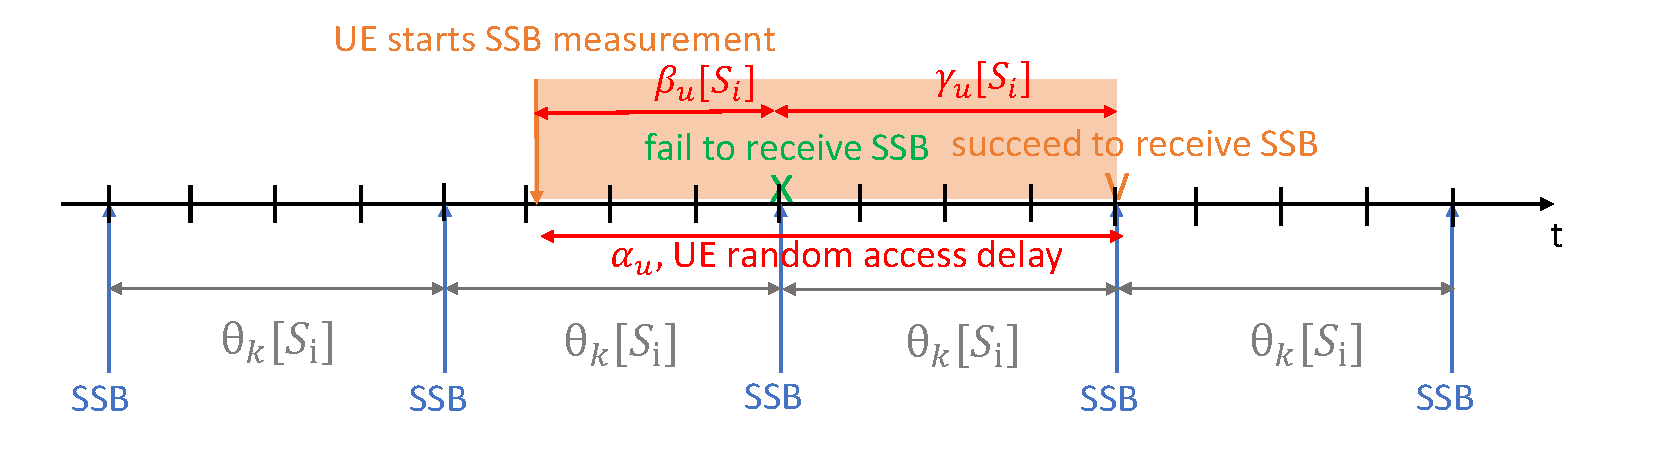
\includegraphics[width=1\textwidth]{figure/random access delay.pdf}
%     \caption{Illustration of UE random access delay. $T_u$ is decomposed into $T_u^i$ (initial waiting time) and $T_u^l$ (additional delay due to failed attempts).}
%     \label{RAD}
% \end{figure}

\section{Problem Formulation}
This section formulates the optimization problem based on recent 3GPP standardization discussions. The main challenge is to provide SSBs to as many cells as possible with limited satellite power. Extending the SSB periodicity for some cells increases UE random access delay, but it saves more power so that there would be other cells to be served. On the other hand, shortening the SSB periodicity reduces the UE cell searching delay, but the serving cells might be less because of the power budget. The transmitted SSB power also affects the success probability of the cell searching delay. The trade-off among power allocation, SSB periodicity, and UE cell searching delay is modeled as follows:

% \begin{equation}
% \begin{aligned}
%     & \underset{P, \theta}{\text{min}} \sum_{u \in \mathcal{U}} \sum_{s \in \mathcal{S}} E[{\alpha_u[s]}] \\
%     & \text{subject to} \\
%     & \quad \sum_{m} P_{m}[t] \leq P^{total}, \quad \forall t \in \mathcal{T} \\
%     & \quad P_{m}[t] \geq 0, \quad \forall m \in \mathcal{M}, t \in \mathcal{T} \\
%     & \quad \theta_k[s] \leq N, \quad \forall k \in \mathcal{K}, \forall s \in \mathcal{S} \\
%     & \quad \theta_k[s] \in \mathbb{N}^+, \quad \forall k \in \mathcal{K}, \forall s \in \mathcal{S} \\
%     & \quad \sum_{k} \frac{1}{\theta_k[s]} \leq M, \quad \forall s \in \mathcal{S} \\ %TODO: explaination of this function
% \end{aligned}
% \end{equation}

\begin{subequations} \label{eq:main}
\begin{align}
    &\min_{P,\,\theta} \sum_{u} \sum_{s\in S} \mathbb{E}[\alpha_u[s]] \\ 
    &\text{subject to} \nonumber \\
    &\sum_{m} \frac{P_{k}[\mathcal{S}_i]}{\theta_k[\mathcal{S}_i]} \leq P^{total}, \quad \forall \mathcal{S}_i \in \mathcal{\widetilde{S}} \label{eq:power_constraint} \\ 
    &P_k[\mathcal{S}_i]\geq 0, \quad \forall k\in\mathcal{K}, \mathcal{S}_i\in\mathcal{\widetilde{S}} \label{eq:power_nonnegative} \\
    &\theta_k[\mathcal{S}_i] \leq N, \quad \forall k\in\mathcal{K}, \mathcal{S}_i\in\mathcal{\widetilde{S}} \label{eq:theta_upper} \\
    &\theta_k[\mathcal{S}_i] \in \mathbb{N}^+, \quad \forall k\in\mathcal{K}, \mathcal{S}_i\in\mathcal{\widetilde{S}} \label{eq:theta_positive} \\
    &\sum_k \frac{1}{\theta_k[\mathcal{S}_i]} \leq M, \quad \forall \mathcal{S}_i\in\mathcal{\widetilde{S}} \label{eq:sum_constraint}
\end{align}
\end{subequations}

where $\mathbb{N}^+$ is the set with all positive integers. The mathematical fomula between transmitted power and received power is described in equation (\ref{eq:T-R}). And the mathematical derivation between the received power $\hat{P}_{m, u}[t]$, $\theta_k[s]$ and $\alpha_u[s]$ is described from equation (\ref{eq:alpha}) to equation (\ref{eq:Ru}). 

% \section{List of Symbols}
% \begin{tabular}{ll}
% \hline
% \multicolumn{2}{l}{\textbf{Symbol}} \\
% \hline
% $N$ & Number of satellites \\
% $M$ & Number of beams per satellite \\
% $K$ & Number of cells on the ground \\
% $U$ & Number of user equipments (UEs) \\
% $L_{n,k}$ & Free space path loss from satellite $n$ to cell $k$ \\
% $h_{n,k}$ & Channel gain between satellite $n$ and cell $k$ \\
% $G(\theta_{n,m,u})$ & Antenna gain for user $u$ \\
% $T^{SSB}_k$ & SSB periodicity of cell $k$ \\
% $T_u$ & Random access delay of UE $u$ \\
% $P_{n,m}$ & Transmitted power of satellite $n$'s $m$-th beam \\
% $P_s$ & Maximum transmitted power for each satellite \\
% $P_{th}$ & SSB reception threshold \\
% $Q_u$ & Number of failed SSB attempts for UE $u$ \\
% \end{tabular}